\documentclass{beamer}  
\usetheme{Warsaw}
\title{Introduction to AI and ML}
\subtitle{Matrix Project}
\author{Ananthapadmanabhan M, EE17BTECH11047 \and \\S.Yogesh, EE17BTECH11039}
\begin{document}

\begin{frame}

\titlepage
 
\end{frame}  

\begin{frame}[t]{Question}

The area(in sq.unit) of the quadrilateral formed by the tangents at the ends of the latera recta of the eclipse $\frac{x^2}{9} + \frac{x^2}{5} = 1$,is:

\vspace{1.5em}

Given eclipse in matrix form:
\vspace{1.5em}

\[x^T
\begin{bmatrix}
1/9 & 0\\
0 & 1/5
\end{bmatrix}
x
=
1
\]

\end{frame}


\begin{frame}{Solution}
Conic equation is matrix form:
\[x^T V x
+
2 u^T x
+
F
=
0
\]
Here,
\[V
=
\begin{bmatrix}
1/9 & 0\\
0 & 1/5
\end{bmatrix}
\]
\[u = O\]
\[
F = -1\]
\end{frame}

\begin{frame}
The length of semi major axis $a = 3$
,the length of semi minor axis $b = \sqrt{5}$
\[F_1 = 
\begin{bmatrix}
\sqrt{a^2 - b^2}\\
0
\end{bmatrix}\]
\[F_2 = 
\begin{bmatrix}
-\sqrt{a^2 - b^2}\\
0
\end{bmatrix}\]
\[F_1 = 
\begin{bmatrix}
2\\
0
\end{bmatrix}\]
\[F_2 = 
\begin{bmatrix}
-2\\
0
\end{bmatrix}\]
\end{frame}
   
\begin{frame}
The end points of the latera recta can be found from
\[
\begin{bmatrix}
2&
y
\end{bmatrix}
\begin{bmatrix}
1/9 & 0\\
0 & 1/5
\end{bmatrix}
\begin{bmatrix}
2 \\ y
\end{bmatrix}
=
1\]
\[
\begin{bmatrix}
-2&
y
\end{bmatrix}
\begin{bmatrix}
1/9 & 0\\
0 & 1/5
\end{bmatrix}
\begin{bmatrix}
-2 \\ y
\end{bmatrix}
=
1\]
From the above equations we get,
\begin{columns}[onlytextwidth]
\column{0.5\textwidth}
\[P_1
=
\begin{bmatrix}
2\\
\frac{5}{3}
\end{bmatrix}
\]
\[P_2
=
\begin{bmatrix}
2\\
-\frac{5}{3}
\end{bmatrix}
\]
\column{0.5\textwidth}
\[P_3
=
\begin{bmatrix}
-2\\
-\frac{5}{3}
\end{bmatrix}
\]
\[P_4
=
\begin{bmatrix}
-2\\
\frac{5}{3}
\end{bmatrix}
\]
\end{columns}
\end{frame}

\begin{frame}
Tangent of a conic is given by
\[(p^T V + u^T) x + p^T u + F = 0\]
Tangent at $P_1$
\[
\begin{bmatrix}
\frac{2}{9} & \frac{1}{3}
\end{bmatrix}
x
=
1
\]
Tangent at $P_2$
\[
\begin{bmatrix}
\frac{2}{9} & -\frac{1}{3}
\end{bmatrix}
x
=
1
\]
Tangent at $P_3$
\[
\begin{bmatrix}
-\frac{2}{9} & -\frac{1}{3}
\end{bmatrix}
x
=
1
\]\\
Tangent at $P_4$
\[
\begin{bmatrix}
-\frac{2}{9} & \frac{1}{3}
\end{bmatrix}
x
=
1
\]
\end{frame}

\begin{frame}
The point of intersection of two lines is given by:
\[x = N^{-T} p\]
Where $N = (n_1 \ n_2)$
Intersection points of tangents at $P_1$ and $P_2$ is
\[
A
=
\begin{bmatrix}
\frac{9}{4} & \frac{9}{4}\\
\frac{3}{2} & \frac{3}{2}
\end{bmatrix}
\begin{bmatrix}
1\\
1
\end{bmatrix}
=
\begin{bmatrix}
\frac{9}{2} \\
0
\end{bmatrix}
\]
\[
B
=
\begin{bmatrix}
\frac{9}{4} & -\frac{9}{4}\\
-\frac{3}{2} & -\frac{3}{2}
\end{bmatrix}
\begin{bmatrix}
1\\
1
\end{bmatrix}
=
\begin{bmatrix}
0 \\
-3
\end{bmatrix}
\]
\[
C
=
\begin{bmatrix}
-\frac{9}{4} & -\frac{9}{4}\\
\frac{3}{2} & \frac{3}{2}
\end{bmatrix}
\begin{bmatrix}
1\\
1
\end{bmatrix}
=
\begin{bmatrix}
-\frac{9}{2} \\
0
\end{bmatrix}
\]
\[
D
=
\begin{bmatrix}
-\frac{9}{4} & \frac{9}{4}\\
\frac{3}{2} & \frac{3}{2}
\end{bmatrix}
\begin{bmatrix}
1\\
1
\end{bmatrix}
=
\begin{bmatrix}
0 \\
3
\end{bmatrix}
\]

\end{frame}

\begin{frame}
Area of quadrilateral formed by tangents,
\[Area = 
4 * Area(\triangle AOB)
\]
\[
Area =
4 * \frac{27}{4}\]
\[Area = 
27
sq. units\]
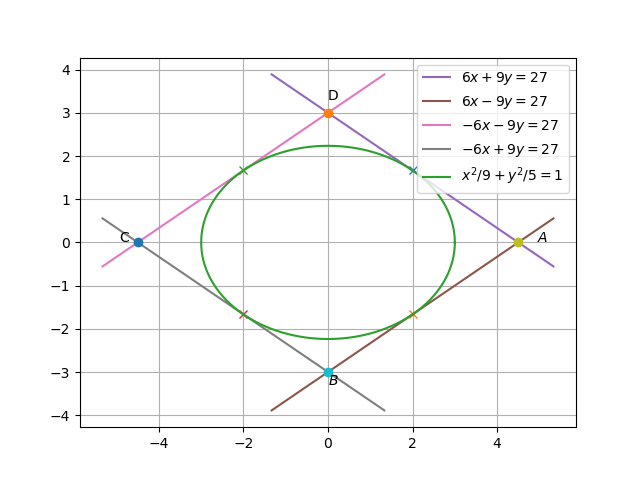
\includegraphics[scale=0.5]{graph}
\end{frame}

\end{document}